
% Experement data + calcs goes here %

\section{Ход работы}

\subsection{Дифракция Френеля на щели}

\begin{enumerate}
    \item Схема установки для наблюдения дифракции Френеля на щели представлена на рис. 1.

    \begin{figure}[h!]
        \center{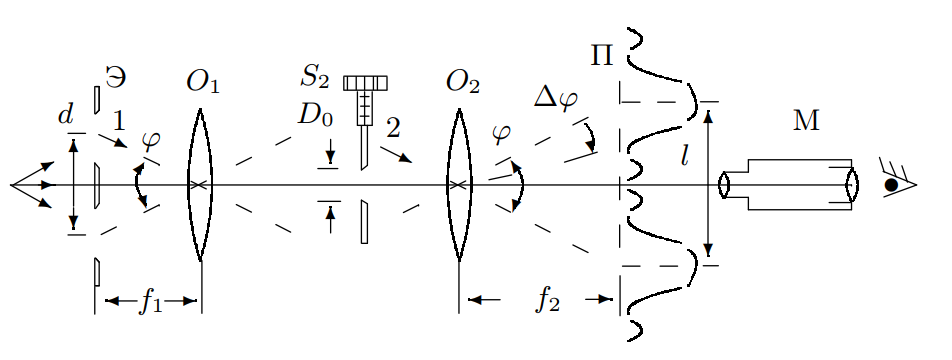
\includegraphics[width = 0.8\textwidth]{picks/scheme1.png}}\\
        \textit{Рис. 1: Схема установки для наблюдения дифракции Френеля.}
    \end{figure}

    \item Проведём настройку приборов, соберём установку. Наблюдаем дифракцию Френеля
    на щели - на ярком фоне изображения щели появляются узкие тёмные полосы, количество
    которых уменьшается по мере удаления микроскопа (дифракция в ближней волновой зоне).

    \item Снимем зависимость координаты микроскопа от числа наблюдаемых полос,
    результаты занесём в таблицу 1.

    \begin{table}[h!]
    \begin{center}
        \caption{Таблица 1.}
        \begin{tabular}{|l|l|l|l|l|l|l|}
        \hline
        Количество темных полос n & 0    & 1    & 2    & 3    & 4  & 5    \\ \hline
        x, мм                     & 52,4 & 49,4 & 50,3 & 50,7 & 51 & 51,2 \\ \hline
        \end{tabular}
    \end{center}
    \end{table}

    \item Сравним размеры зон Френеля с измеренной шириной $D\ruB{щели} = 340\pm5$ мкм $S_2$.
    Для этого рассчитаем величину $2z_n=2\sqrt{an\lambda}$($\lambda = 579$ нм). Тогда
    $D = \frac{1}{5}\sum_{n = 1}^{5}  2z_i = 330\pm6$ мкм.

\end{enumerate}

\newpage

\subsection{Дифракция Фраунгоффера на щели}

\begin{enumerate}
    \item Схема установки для наблюдения дифракции Фраунгоффера представлена на рисунке 2.

    \begin{figure}[h!]
        \center{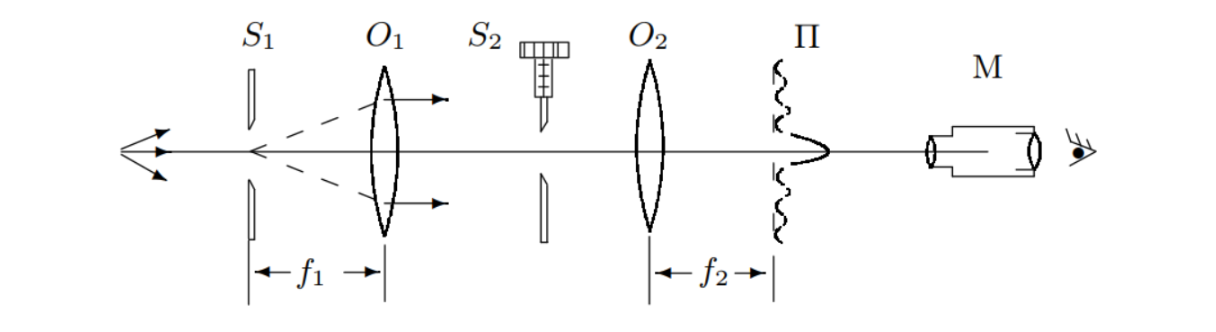
\includegraphics[width = 0.8\textwidth]{picks/scheme2.png}}\\
        \textit{Рис. 2: Схема установки для наблюдения дифракции Фраунгоффера.}
    \end{figure}

    Фокусные расстояния линз F1 = 11,5 см, F2= 12,8 см. Ширина щели $D=400\pm5 $мкм.

    \item Измеренния представлены в таблице 2.

    \begin{table}[h!]
        \begin{center}
            \caption{Таблица 2.}
            \begin{tabular}{|l|l|l|l|l|l|l|l|l|}
            \hline
            m & -4 & -3 & -2 & -1 & 1 & 2 & 3 & 4 \\ \hline
            $x_m$, мм & 0,08 & 0,1 & 0,12 & 0,14 & 0,17 & 0,19 & 0,21 & 0,23 \\ \hline
            \end{tabular}
        \end{center}
        \end{table}

    \item График представлен на рисунке 3.
    
    \begin{figure}[h!]
        \center{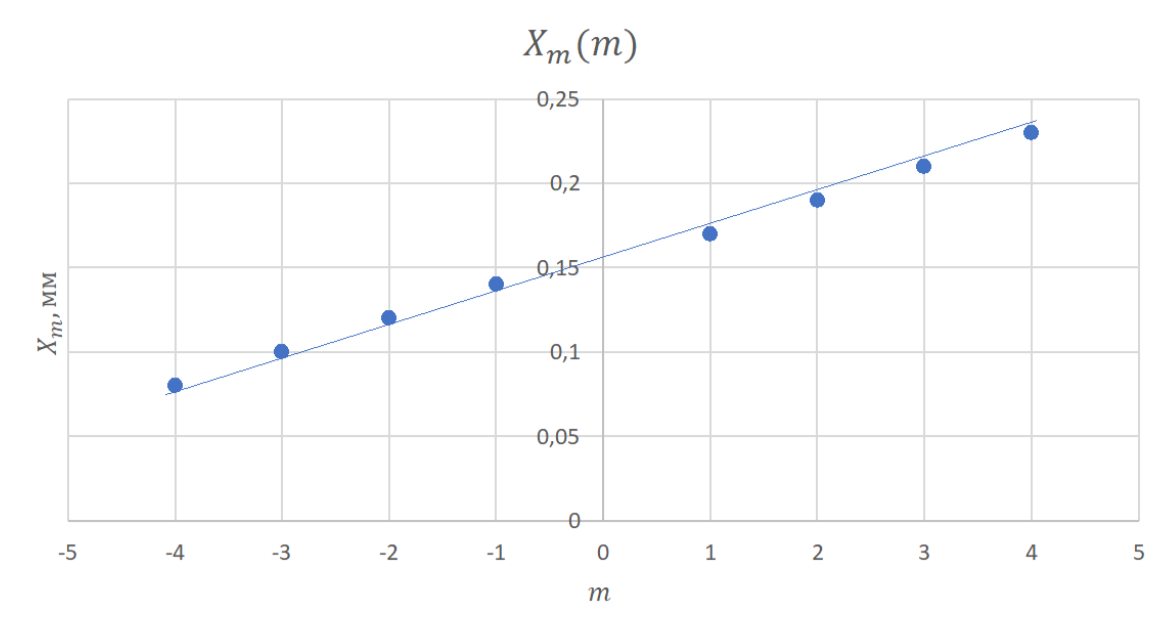
\includegraphics[width = 0.8\textwidth]{picks/graph.png}}\\
        \textit{Рис. 3: График для дифракции Фраунгоффера.}
    \end{figure}

    \item Посчитал D по МНК: $D = 402\pm8$ мкм

\end{enumerate}

\newpage

\section{Вывод}

Были получены интерефереционные картины для дифракции Френеля и Фраунгофера.
Теоретические формулы были успешно проверены на практике.